\documentclass[runningheads]{llncs}

\usepackage{graphicx}
\usepackage{booktabs}
\usepackage{amsmath}
\usepackage{siunitx}

% Package for todo command
\usepackage{xcolor}

\newcommand\todo[1]{\textcolor{red}{#1}}

\begin{document}

\title{ActiVis: Mobile Object Detection and Active Guidance for People with Visual Impairments}
\titlerunning{Mobile Object Detection and Active Guidance}

\author{J.C. Lock\inst{1} \and
  G. Cielniak\inst{1} \and
  A.G. Tramontano\inst{2} \and
  N. Bellotto\inst{1}
}
\authorrunning{Jacobus C. Lock et. al.}
\institute{University of Lincoln, Lincoln, UK \and
  Universit\`{a} degli studi di Padova, Italy
}

\maketitle

\begin{abstract}
  The ActiVis project aims to deliver a system for a mobile device that is able to guide a person with visual impairments towards a target object or area in an unknown indoor environment. 
  To do so, it uses new developments in object detection methods, mobile computing, action generation and human-computer interfacing to interpret the user's surroundings and present useful guidance directions.
  Our approach to action generation used a Markov Decision Process (MDP) to track the system's state and output the next best location to investigate to find a target object and has been shown to work in principle in~\cite{lock2019active}.
  This work expands upon that by adding an object detector and adapting the decision-making process accordingly, providing a complete object search and guidance pipeline.
  The improved ActiVis system was evaluated in a set of experiments and it outperformed the baseline, unguided case.
  \keywords{Active vision, vision impairment, object detection}
\end{abstract}

\section{Introduction}

There are an estimated half a billion people that live with mild to severe vision impairment or total blindness and this number is expected to significantly rise with an ageing population~\cite{bourne2017magnitude}.
There has been a rise interest from industrial partners in utilising modern technology to make their products more accessible and improvements in modern computing power and image processing capabilities have made this easier.
The work we present here is part of the ActiVis project that aims to assist people with vision impairments (PwVI) to independently navigate and find objects within an unknown indoor environment using only a mobile phone and its camera.
This system implements active vision ideas~\cite{bajcsy2017}, but replaces the electro-mechanical servo typically found in active vision systems with a user's arm and hand as pictured in Fig.~\ref{fig:system-in-use}.
This project expands upon concepts proposed in~\cite{bellotto2013,lock2017portable} and builds off of the system introduced in~\cite{lock2019active}.

\begin{figure}
  \centering
  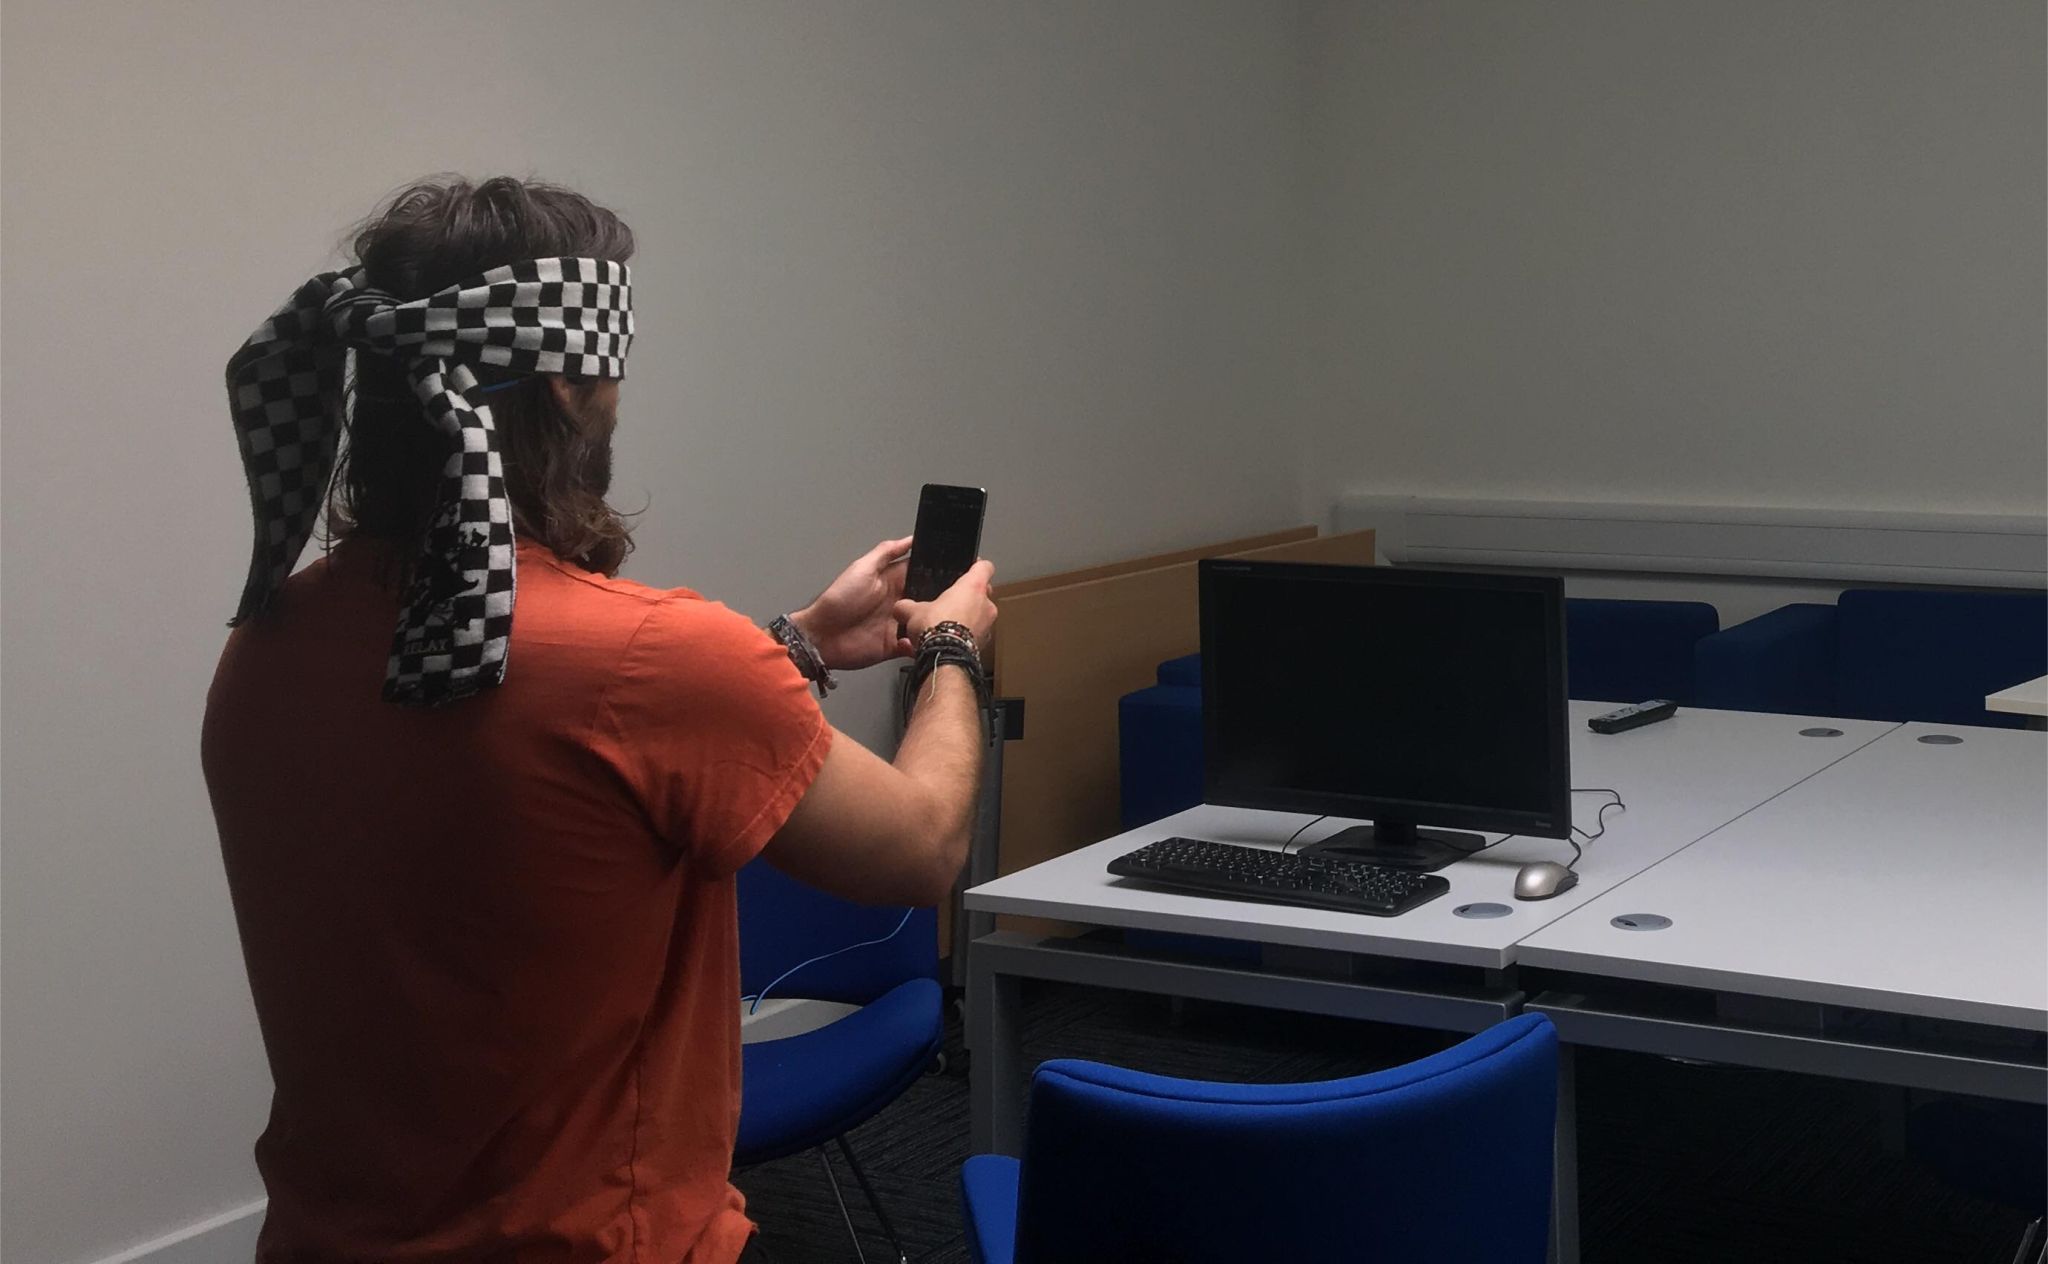
\includegraphics[width=0.5\textwidth]{figures/system_use.png}
  \caption{The system in use during an experiment with a blindfolded participant. }\label{fig:system-in-use}
\end{figure}

ActiVis uses the camera's current and previous image data as input and leverages its understanding of inter-object spatial relationships to determine the best navigation action to take to reach the target object.
To enable this, we expanded upon our previous work and implemented a partially observable Markov Decision Process (POMDP)~\cite{bellman1957markovian} on a mobile phone that generates real-time navigation instructions to guide the user to their target object.
This work makes the following contributions:

\begin{itemize}
  \item a controller that enables object search and guidance on a mobile phone;
  \item a complete system pipeline that includes interfacing, object detection and human control;
  \item experiments that evaluate the efficacy of the proposed system.
\end{itemize}

Section~\ref{sec:previous-work} discusses relevant previous work, followed by a description of the active vision system and human controller in Sections~\ref{sec:active-vision} and~\ref{sec:human-controller} respectively. 
The experiments that were conducted in this work and their results are discussed in Sections~\ref{sec:experiments} and~\ref{sec:results}, followed finally by a short conclusion and discussion of the next steps for the project in Section~\ref{sec:conclusion}.

\section{Previous Work}\label{sec:previous-work}

%Mobile devices that can detect objects and guide PwVI in real-time using on-board processing power has become more feasible in recent years thanks to improvements in mobile computing and image processing methods.
Early attempts to solve this guidance problem used markers encoded with object or environmental information and a smartphone that scans the environment for these simple patterns~\cite{gude2013blind,manduchi2012mobile}. 
The device uses a feedback mode (e.g.\ voice, Braille) to read out the embedded information or guide the user towards the markers. 
Improvements to feature detectors have made it viable~\cite{redmon2016you,huang2017speed} to replace markers with real objects while providing the same guidance functionality.
%The SIFT based system in~\cite{schauerte2012assistive} is an example of a markerless system.
An alternative detection approach proposed in~\cite{bigham2010vizwiz} requires the user to send a photo of their environment to a Mechanical Turk worker that sends the position of the requested object within the picture back to the user. 

The issue with a marker-based approach is that it requires significant effort to place and maintain them in an environment, which is remedied by markerless systems.
However, both of these approaches are passive in their guidance approach and rely on the user placing the desired marker/object within the camera's view by themselves before any guidance is provided. 
The system in~\cite{bigham2010vizwiz} can leverage a human's understanding of the environment to help guide a user to the correct location, but the there is significant lag and a reliance on a good internet connection and remote worker being available. 
Our previous work on the ActiVis system~\cite{lock2019active} addressed the passive guidance issue by implementing an MDP-based controller that provides the user with pointing instructions to find an out-of-view object and proved that this is a viable method to search for an object. 
However, this work used barcodes encoded with object information to simulate real objects.
In this work, we are replacing the barcodes with real objects, thereby providing a complete object detection and guidance pipeline. 

Object detectors mainly come in 2 flavours: 2-stage models that use an external algorithm to select regions of interest to perform object inference on~\cite{ren2015faster}, and single-stage models that generate multiple, differently-sized windows and checks each window for any objects.
Between the 2 types, there is a speed-accuracy tradeoff, where 2-stage models typically produce more accurate results, but are slower and require more computing resources~\cite{liu2018deeplf}.
On the other hand, single-stage models, such as SSD, YOLO and MobileNet~\cite{liu2016ssd,redmon2018yolo,howard2017mobilenet} produce less accurate results, but with drastically less parameters and FLOPS required to perform object inference than the 2-stage models. 
%MobileNet~\cite{howard2017mobilenet} in particular is a 2-stage network designed specifically for mobile platforms with moderate precision levels, but can reach around 10 frames per second on a mobile platform.
%The two-stage models, such as Faster R-CNN~\cite{ren2015faster}, use a region proposal network approach where an external algorithm proposes a region of interest that the classifier uses as input to recognise any objects. 
%They typically reach higher accuracy, but at the cost of increased memory and computational resource requirements~\cite{liu2018deeplf}.
%On the other hand, single-stage methods apply multiple differently sized windows over the image and checks if any objects appear in those windows. 
%These methods, such as Single-Shot Detection (SSD)~\cite{liu2016ssd} and You Only Look Once (YOLO)~\cite{redmon2018yolo}, typically need less computational resources, but at the cost of decreased accuracy.
%Marrying a single-stage method to a feature extractor yields higher accuracy, by at the cost of increased computational resources. 
%There is therefore a fine speed-accuracy trade-off to be made, particularly in a mobile context where processing resources are limited. 
%MobileNet~\cite{howard2017mobilenet} is a classifier network that can be used as a feature extractor  that introduced depth-wise separable convolutions that decrease the number of operations needed to make a convolution.
%This leads to model that uses much less memory, but again with a small drop in accuracy.

\section{Active Vision System}\label{sec:active-vision}

The ActiVis project's goal is developing a mobile system that can guide a PwVI towards their desired destination with minimal user input or intervention. 
%This work focuses on guiding a user towards an object in one static environment and is limited to 2 dimensions (pan and tilt).

A complete system diagram is given in Fig.~\ref{fig:sys-diagram}. 
This diagram shows a typical feedback control loop that generates a control signal to minimise some error signal, but has been modified to incorporate a human within the loop.

\begin{figure}
  \centering
  \includegraphics[width=0.75\textwidth]{figures/control_loop.png}
  \caption{The system control loop including a human and the controller.}\label{fig:sys-diagram}
\end{figure}

In this case, the error, $e$, is defined as the difference between the desired object and the object currently within view. 
The implication of adding a human into the loop is that an additional block, \emph{H}, is added to simulate a human that receives an control signal, \emph{u}, from the controller, \emph{K}. 
However, the challenge with people is that a person may interpret \emph{u} in any unpredictable way (i.e.\ apply a transformation) that results in the signal \emph{u*} that points the camera, \emph{P}, to a new location containing a new object observation, \emph{y}.
It is therefore important to design \emph{K} to be robust enough to accommodate different user habits and limitations and ensure that \emph{u*} tracks \emph{u} as closely as possible. 
%These design considerations are addressed in previous work. \todo{how to state that we designed the interface already if its unpublished?}

Another fact to take note of is the measurement noise, \emph{n}, added in the feedback loop that simulates an object detector's classification errors that influence the action that \emph{K} generates. 
In our previous work, we assumed a perfect classifier and solved the problem using a Markov decision process (MDP). 
In this work we do away with that somewhat naive assumption and implement a POMDP that can handle classification uncertainties in object detectors and classifiers. 

\section{Human Controller}\label{sec:human-controller}

The POMDP controller that we implemented for this work is an extension to the MDP-based controller we made for the experiments described in~\cite{lock2019active}.
It works by generating a trail of virtual waypoints for the user to point the camera towards that eventually leads to the target object.
The waypoint positions are based on the model's pre-trained internal knowledge of the inter-object spatial relationships and they are placed in a way that maximises the probability of the user finding the target object.
%A new waypoint is generated when the user finds the current waypoint or finds another ancillary object.

\subsection{Design}

A POMDP is an extension to the MDP model that allows it to handle cases where the state is not directly observable, allowing it to be used in more realistic scenarios. 
%In this case, the state is inferred based on the model parameters and the associated sensor accuracy (if a sensor is 100\% accurate, the state would be directly observable).
The implication of this is that a POMDP-based agent does not know its state at any point in time, but must infer it based on the known model parameters and sensor accuracy, the object detector's accuracy in this case.
This state inference relies on a so-called belief meta-state that is updated with additional observations to reflect the likelihood that the agent is in any given state.
The belief state is fully observable by the agent and can be used to infer the mobile device's current state and generate the next action.

A POMDP model is represented by the 8-tuple $(\mathbf{S}, \mathbf{A}, \mathbf{T}, \mathbf{R}, \mathbf{\Omega}, \mathbf{O}, \mathbf{b}, \gamma)$, where $\mathbf{S}$ represents a finite set of discrete states, $\mathbf{A}$ is a set of discrete actions, $\mathbf{T}$ is a matrix containing the probabilities of transitioning from state $s$ to state $s'$, $s, s' \in \mathbf{S}$, after executing action $a$, $a \in \mathbf{A}$, and $\mathbf{R}$ is the reward the agent receives executing action $a$ and reaching state $s'$.
$\mathbf{\Omega}$ is the set of possible state observations, while the matrix $\mathbf{O}$ contains the probabilities of making state observation $\omega$, $\omega \in \mathbf{\Omega}$, when in state $s$ after executing action $a$.
Finally, $\mathbf{b}$ is the belief vector containing the state probability distribution and $\gamma$ is a discount factor that prioritises long-term over short-term rewards and affects the model's convergence rate. 
%$\mathbf{b}$ is updated for every timestep and action-observation pair.
Each of the POMDP's parameters are discussed next. 
%This update is done with

%\begin{equation}
  %b_t(s') = \eta\Omega(o, s', a)\sum_{s\in\mathbf{S}}\mathbf{T}(s, a, s')b_{t-1}(s), 
%\end{equation}
%where $\eta$ is a normalisation factor. 

%The state space, reward function and transition matrix are conceptually similar the same as the MDP described in~\cite{lock2019active}. 
%The major difference is the addition of an observation matrix that defines the probability of being in any given state after making a new observation.
%In essence, it is a measure of the sensor accuracy, and in this case it describes the object detector's classification accuracy and recall.
%These parameters are given by the following. 

\subsubsection{State Space}

The state is given by $s = \langle u, n, v \rangle$, where $u, u\in\mathbf{U}$, is the object within view, n the number of search steps taken since the search began and a binary variable $v$ that tracks the uniqueness of a waypoint's position for the search.

\subsubsection{Actions}

The possible actions that dictates the location the mobile device will generate the next waypoint are given by $\mathbf{A} = \{ \textrm{UP, DOWN, LEFT, RIGHT} \}$.

\subsubsection{Transitions}

$\mathbf{T}$ was determined by extracting the inter-object spatial relationships for a limited number of objects in terms of the actions in $\mathbf{A}$ from the OpenImages~\cite{openimages} dataset. 
For example, by iterating over the images containing the objects of interest, we can see that the object `monitor' is located above (i.e. UP) the object `keyboard' in 16\% of images containing both objects (see Fig.~\ref{fig:openimage}). 
The transition function for this case is $t(s, a, s') = t(\textrm{keyboard}, \textrm{UP}, \textrm{monitor}) = 0.16$.

%\begin{equation*}
  %t(s, a, s') = t(\textrm{keyboard}, \textrm{UP}, \textrm{monitor}) = 0.16.
%\end{equation*}
%An image displaying this relationship can be seen in Fig.~\ref{fig:openimage}.

\begin{figure}
  \centering
  \includegraphics[width=0.5\columnwidth]{figures/desk_example.png}
  \caption{An example from of an image from the OpenImage dataset~\cite{openimages} containing typical office objects}\label{fig:openimage}
\end{figure}

\subsubsection{Reward Function}

The reward function encourages the device controller to search for and find the target object by giving it a substantial reward for doing so, while penalising it for every action that does not result in it finding the target object.
Furthermore, additional penalties are given if the controller generates a waypoint in an area it has explored before $(v = \textrm{true}$) or when it exceeds some search length threshold denoted by $n_{\max}$.
The rewards are summarised in Table~\ref{tab:rewards}.

\begin{table}
  \centering
  \caption{The reward function for the POMDP. }\label{tab:rewards}
  \begin{tabular}{p{3cm}p{1cm}}
    \toprule
    $r(o = o_{target})$ & 10000 \\ \midrule
    $r(v = \textrm{true})$  & -75 \\ \midrule
    $r(n > n_{\max})$ & -75 \\ \midrule
    otherwise $r(\cdot)$ & -100  \\ \midrule
    \bottomrule
  \end{tabular}
\end{table}

\subsubsection{Observations and Observation Matrix}

The state observations are identical to the states that the mobile device can enter. 
In this case, however, uncertainty is introduced into the observation by the object detector.
Previous search locations and search time are fully observable here, since they can be tracked by the mobile device.
$\mathbf{\Omega}$ therefore only contains the classification/misclassification probabilities of the object detector. 
These values were found by performing a set of classifier tests on the object detector and generating a confusion matrix to populate $\mathbf{\Omega}$.

\subsubsection{Training}

We encoded 16 objects, including a `nothing' object where the detector does not see anything of interest, into the controller and object detector.
These objects are defined as 

\begin{equation*}
  \begin{split}
    \mathbf{U} = \{ nothing, monitor, keyboard, mouse, desk, laptop, mug, window,\\ 
      lamp, backpack, chair, couch, plant, telephone, whiteboard, door \}.
  \end{split}
\end{equation*}

\noindent We set $n_{\max}$ to 12 waypoints, after which the agent gets penalised for every additional waypoint it generates that does not lead to the target object. 
This results in a total of 352 reachable states ($n_{states} = 16\times11\times2$), with any state containing the target object acting as a terminal state.

The POMDP model is put through a training process to generate a policy that contains the optimal belief-action mapping that the controller can use to produce the optimal waypoint locations.
This is done by having the model explore the entire state-action-observation space and optimising the policy to maximise its long-term cumulative reward.
The difficulty of solving POMDPs is that $\mathbf{b}$ is a vector of continuous probability distributions with infinite combinations, making POMDPs time-consuming or even impossible to solve exactly.
We found this to be the case for our moderately-sized state space size and therefore opted to use an approximate method instead.
Multiple algorithms have been proposed~\cite{bargiacchi2016dynamic,silver2010monte} and in this work we used the Point-Based Value Iteration (PBVI) algorithm~\cite{pineau2003point} as implemented in the AI-Toolbox library~\footnote{github.com/Svalorzen/AI-Toolbox} to solve the POMDP model.
The PBVI algorithm speeds up the optimisation process by selecting a smaller subset of representative belief points from the belief function and tracking these points only. 
Using the PBVI algorithm, we generated a total of 15 policies, one for each target object. 

\subsection{Guidance System Implementation}

We implemented the object detector and POMDP controller by combining it with an audio interface that provides non-visual guidance instructions onto an Android app.% that can be used by a PwVI by adding .% onto a mobile phone that can generate and provide guidance instructions for a user.  
Non-visual feedback allows the app to be used by PwVI.
%This was done by combining an audio interface that provides non-visual guidance instructions, the POMDP controller and object detector onto a mobile app.
Each of these aspects and their implementation are discussed here.

\subsubsection{Audio Interface}

ActiVis's target audience are PwVI and therefore provides guidance instructions in a non-visual manner that is intuitive and easy to understand. 
To avoid blocking a user's access to ambient sounds, we use a set of non-intrusive bone-conducting headsets to transmit the audio signals to the user. 

To describe the waypoints' pan and tilt positions, we implemented an improved version of the interface described in~\cite{bellotto2013} that uses a spatialised audio signal.
However, since our headphones bypass the ear's pinnae that allow a person to localise the height~\cite{roffler1968factors}, we spatialise the audio in the pan dimension only.
To convey the tilt angle, we instead exploit a human's natural association of high and low sound sources with a high and low sound frequency respectively~\cite{blauert1997spatial} and adjust the sound source's pitch accordingly. 
A similar approach was used in~\cite{schauerte2012assistive}.
With this interface and headset, ActiVis is able to describe location of a waypoint to a user in the pan and tilt dimensions.

\subsubsection{Object Detector}

SSD-Lite is a single-stage object detection and classification network that is based on the SSD architecture that implements MobileNetV2~\cite{sandler2018mobilenetv2}.
This is a lightweight model that requires relatively little memory to perform inference tasks, making it suitable for mobile platforms. 
This model achieves a mAPs of 0.22 with 4.3M parameters and 0.8B FLOPS~\cite{li2018tinydsod} on the COCO dataset~\cite{lin2014microsoft}. 
The full SSD model achieves a slightly higher mAPs (0.25), but with significantly more parameters (34.3M) and FLOPS (34.36B).
Tiny-DSOD~\cite{li2018tinydsod}, an alternative to SSD-Lite, has similar precision and computing requirements (mAPs=0.23, parameters=1.15M, FLOPS=1.12B), but we found that SSD-Lite produced better results for this application and chose to implement it in ActiVis.

The network was trained with a maximum of 10000 object samples, taken from the OpenImages dataset~\cite{openimages}, for each object class in $\mathbf{U}$ with a 60\%/20\%/20\% split for training, validation and testing respectively.
We set a relatively high confidence threshold of 0.7 to reduce the likelihood of false-positives.
With 120 training epochs with 1000 iterations each, we achieved a mAPs of 0.16 on this dataset and produced a TensorFlow Lite model that is compatible with Android. 
%We also built our own test small dataset to test the model with.\todo{should we include this? Doesnt look very good}
%This dataset contains 459 images for each of the objects in $\mathbf{U}$ in different sizes and orientations and the objects used were the same objects that were used in the experiments. 
%\todo{add mAPs we achived}

\subsubsection{Action Generator}

The output from the POMDP model's training process is a policy file that defines the best location to place the next search waypoint based on the device's current state.
This state is tracked by the device throughout the app's runtime by performing object detection and recording the device's previous search locations and previous waypoint positions
The latter is done by disretising the world into a $6\times6$ grid and setting the relevant grid unit's $v$ value.
Each grid square represents a \SI{35}{\degree} angular translation and the grid encompasses a \SI{210}{\degree}$\times$\SI{210}{\degree} field of view. 
This setup gives the state access to perfectly observable $n$ and $v$ parameters, while $o$ is generated by the object detector. 

When the device makes a new state observation, $\omega$, either because the user rotates the device past \SI{35}{\degree} or sees a new object, the device triggers the controller to generate a new waypoint location.
The controller uses $\omega$ to update $\mathbf{b}$ and queries the policy for the best location to place the new waypoint. 
The policy output is an action from $\mathbf{A}$ that indicates the next adjacent grid square to place the waypoint, e.g.\ `UP' output would result in a waypoint being placed one grid square above the grid square within view. 

\section{Experiment Design}\label{sec:experiments}

To evaluate the guidance system's effectiveness, we designed a set of experiments to measure its performance in driving a user towards a target object within a static environment. 
We conducted an additional set of experiments with an alternative guidance system to act as a baseline measurement for our system's results. 
This alternative system does not provide any guidance instructions to the user.
Instead, it provides the user with raw observations from the object classifier and relies on the user's intuition and prior knowledge to generate actions. 
%The goal of both the guided and unguided experiment cases were to find an object within a static environment. 

We recruited 10 participants (8 male, 2 female; average age 29.2 years) for the experiments, including 2 legally blind participants. 
The other 8 participants were blindfolded to simulate blindness. 
The app was run on an Asus ZenPhone AR with Android 7.0 and ARCore~\footnote{developers.google.com/ar/} and text-to-speech enabled. 

\subsection{Unguided Case}

The goal of this experiment is to mimic a typical person with healthy eyesight's search behaviour. 
In such a scenario, a person would see the objects currently within their field of view and use their prior knowledge and intuition to make a decision on where to look next.
For example, a person in bathroom facing the basin after washing their hands is unlikely to find a hand dryer placed above or below the basin so it is reasonable to believe that they would instinctively look at chest height on the walls to their left, right or behind them instead. 

For this experiment, the mobile camera and object detector acts as the participants' eyes and informs them about the objects within the camera's view.
It is then up to the participant to exploit their prior knowledge and intuition to manipulate the camera and find the target object. 
This process is modelled by the schematic in Fig.~\ref{fig:sys-diagram-no-controller} where the human acts as both the actuator and controller.
The app only reads out the objects upon the user's request by tapping on the screen. 
When the target object comes within the camera's view and is correctly detected, the device vibrates to inform the participant. 

\begin{figure}
  \centering
  \includegraphics[width=0.5\textwidth]{figures/control_loop_no_controller.png}
  \caption{The control loop with the human acting as bot manipulator and controller. }\label{fig:sys-diagram-no-controller}
\end{figure}

Each participant was verbally informed prior to each experiment what the target object was and they were given 45 seconds to find it and each run was ended when a target was found or the time limit was reached. 
The learning effect was ignored in order to mimic the normal search behaviour described earlier and allow full use of prior knowledge. 
This process performed once for each object in the experiment set. 

\subsection{Guided Case}

In this experiment, we evaluate the performance of the guidance system in an object search task, where the perception and control tasks are performed by the guidance system and the participant acts as the actuator, interpreting control signals and outputting actuation forces on the camera sensor. 
This is modelled in the schematic in Fig.~\ref{fig:sys-diagram}. 

The participants were not told what the targets objects were in this experiment to eliminate the possibility of them ignoring the guidance instructions in order to try and find the target object faster themselves.
This also isolated the performance measurement to the guidance system alone.
An experiment run started with the experiment staff selecting the target and was terminated when the target object was found or the 45 second time limit was reached.
This process performed once for each object in the experiment set. 

\subsection{Environment Setup}

The environment and the object placement within it for both experiments was modelled on a typical office.
Measures were taken to ensure that both office environments were unique in layout and object placement. 
However, for the larger, more static objects (e.g.\ a desk or door) there is cross-experiment occurrences, which is not a problem since most offices contain the same basic furniture and objects. 
These objects were placed in different locations relative to each other for the 2 experiments to minimise any learning effects that may occur between the experiments. 
The objects in the guided experiment environment are

\begin{equation*}
  \mathbf{u}_{guided} = \{ door, desk, chair, whiteboard, mouse, laptop, backpack, mug \},
\end{equation*}
while the objects in the unguided experiment are

\begin{equation*}
  \mathbf{u}_{unguided} = \{ door, desk, chair, whiteboard, mouse, monitor, telephone, keyboard \}.
\end{equation*}
%A picture of the unguided experiment environment is given in Fig.~\ref{fig:experiment-env}. 

%\begin{figure}
  %\centering
  %\includegraphics[width=0.7\textwidth]{figures/environment.png}
  %\caption{A picture of the experiment setup. }\label{fig:experiment-env}
%\end{figure}

\section{Results}\label{sec:results}

\subsection{Target Acquisition}

%We set an upper time limit for each object search run of 45 seconds.
%When this upper threshold was reached, the search was recorded as a failure and the next run was started. 

The target acquisition rate (TAR) is the proportion of objects the participants successfully found during an experiment. 
For example, a TAR of 0.5 indicates that a participant found the target object in 50\% of searches. 
Taking each participant's TAR as a datum, we found the unguided case produced a higher average TAR (0.54 vs. 0.46), meaning that a participant found around 8\% more objects without guidance instructions.
However, the Kruskal-Wallis (KW) test for non-normal data shows that these results are statistically not significantly different from one another ($p_{kw} = 0.16$), meaning we cannot conclude which experiment produced the best TAR. 
All the experiment results are summarised in Table~\ref{tab:results}. 

\begin{table}
  \centering
  \caption{A summary of the experiment results. }\label{tab:results}
  \begin{tabular}{p{5cm}p{2cm}p{2cm}p{2.5cm}}
    \toprule
    & \textbf{Guided} & \textbf{Unguided}  & \textbf{KW Statistic} \\\midrule
    TAR [\%]           & $46\pm13$ & $54\pm15$ &  0.16 \\\midrule
    Time to target [s] & $12.5\pm11.9$ & $17.2\pm11.5$ & 0.045 \\\midrule
    Pan Angle Displacement [rad] & $0.68\pm1.1$ & $0.99\pm1.2$ & 0.029 \\\midrule
    Tilt Angle Displacement [rad] & $0.68\pm1.1$ & $1.04\pm1.2$ & 0.011 \\\midrule
    Linear Displacement [rad] & $0.23\pm0.22$ & $0.36\pm0.22$ & 0.012 \\\midrule
    \bottomrule
  \end{tabular}
\end{table}

\subsection{Time to Target}

%\todo{Should I add CDF?}
The time it takes to find a target object is an important indicator of system performance, where less time indicates a shorter search time and increased performance.
The data for the search times for each experiment are shown in Fig.~\ref{fig:boxplot-time}.%, while Fig.~\ref{fig:cum-time} shows the cumulative distribution functions (CDF) for the search times as a function of the total number of objects found.

\begin{figure}[h]
  \centering
  \includegraphics[width=0.7\textwidth]{figures/boxplot_time_to_target.png}
  \caption{A set of boxplots comparing the time to target for each experiment. }\label{fig:boxplot-time}
\end{figure}

%\begin{figure}
  %\centering
  %\includegraphics[width=0.7\textwidth]{figures/cumplot_time_to_target.png}
  %\caption{A set of CDFs comparing the time to target. }\label{fig:cum-time}
%\end{figure}

%To compensate for the different numbers of targets found per participant and for each experiment setup, we average each participant's results, giving us 10 samples per experiment. 
From Fig.~\ref{fig:boxplot-time}, it can be seen that the guidance system reduced the overall time it took the participants to find each target object.
This is confirmed by the data that show an average search time of 12.5s for the guided experiment and 17.2s for the unguided case ($p_{kw}=0.045$), an improvement of around 27\%.
%These results are summarised in Table~\ref{tab:results}. 
%With this 27\% reduction in total time spent searching for a target object, we can conclude that a user benefits from using our smart guidance system as opposed to relying on a simple object reader. 
%This is supported by the CDFs in Fig.~\ref{fig:cum-time} that show that \todo{Discuss the less number of objects found and how it is not statistically signioficatn. Perhaps show it in CDF}

\subsection{Movement}

To give an indication of the effort required to find each target, we look at the mobile device's displacement data. 
In this case, less device displacement is desirable, since it implies less physical exertion was demanded from the user.%, enhancing user experience and improving ease of use.
%\todo{maybe cite paper that says less exertion is good}.

The device displacement was measured in both linear ($x, y, z$) and angular (pan, tilt) dimensions.
By integrating these data we obtain and compare the total absolute displacement in each dimension.
These results are plotted in Fig.~\ref{fig:boxplot-displacement}.

%\begin{figure}
  %\centering
  %\includegraphics[width=0.7\textwidth]{figures/boxplot_angle.png}
  %\caption{A set of boxplots comparing the angular distance the device travelled for each experiment. }\label{fig:boxplot-angle}
%\end{figure}

%\begin{figure}
  %\centering
  %\includegraphics[width=0.7\textwidth]{figures/boxplot_dist.png}
  %\caption{A set of boxplots comparing the distance the device travelled for each experiment. }\label{fig:boxplot-dist}
%\end{figure}

\begin{figure}[h]
  \centering
  \includegraphics[width=0.8\textwidth]{figures/boxplot_displacement.png}
  \caption{A set of boxplots comparing the linear and angular displacement the device travelled for each experiment. }\label{fig:boxplot-displacement}
\end{figure}

The boxplots for the total angle displacement show a consistent reduction in radians for the guided case for both the pan (\SI{0.68}{\radian} vs. \SI{0.99}{\radian}, $p_{kw}=0.029$) and tilt dimensions (\SI{0.68}{\radian} vs. \SI{1.05}{\radian}, $p_{kw}=0.011$). 
The guidance system therefore reduces the total angular displacement to find the objects by 31\% and 35\% for the pan and tilt dimensions respectively. 
The total linear displacement is also reduced when using the guidance interface by approximately 36\% (\SI{0.23}{\metre} vs. \SI{0.36}{\metre}, $p_{kw}=0.012$).
These results are summarised in Table~\ref{tab:results}.
To conclude, the data show that the guidance interface reduced the total angular and linear displacement required to find the target objects in all dimensions by at least 31\%, reducing the total effort required by the user. 

\section{Conclusion}\label{sec:conclusion}

In this work, we presented ActiVis, a mobile guidance system that uses an object detector to scan the environment for objects and a POMDP-based controller and audio interface to generate and present the user with guidance instructions. 
We implemented this system on an Android app and tested it with a group of 10 participants to evaluate its effectiveness compared to a baseline, unguided case that only uses the object detector and relies on the human to generate the search path. 
The key results from these experiment is that the guidance system improved the participants' target-searching performance, reducing the total search time and overall camera manipulation effort required when compared to a base case.
However, the participants were able to find 8\% more objects on average in the unguided case, but this result was found to be statistically insignificant. 
With these results, we can reasonably conclude that our system enables a blind or blindfolded user to find a target object and does so better than the alternative base case.

The next steps for the project are to refine and expand the object detector to include objects from other environments. 

\bibliographystyle{splncs04}
\bibliography{bib}

\end{document}
